\section{予備実験}
口から鼻に抜ける香り(オルソネーザル)からの嗅覚情報の提示方法として,アガーを使用し
たゼリーを用いた.アガーを使用したゼリーを球体に固め,その中身を空洞にすることで空気を
入れるスペースが出来る.スペースに香りを閉じこめることで香りを閉じこめたゼリーを作成し
た.そのゼリーを口から食べることで口の中でゼリーが割れることにより,閉じこめられていた
香りが出て鼻から抜ける香りを与える物となっている.

\subsection{球体ゼリーの作成方法}
中に香りを閉じこめるためには,ゼリーの中身を空洞にする必要がある.そのため,ゼリーを
作成するための材料といてアガーを使用した.今回アガーを利用した理由は,ゼラチンよりも透
明度が高く,常温でも溶けない性質を持っているからである.また,アガー自体には味がついてお
らずゼリー状に固めても無味無臭で作ることが出来る.もう一つの特徴として,溶ける温度が 90
℃以上と溶けにくく,固まる温度が 30,40 ℃と常温でも固まりすぐに固めることが出来るため
扱いやすく丈夫である.固める際に図 4.1 で示した丸い氷を作成する用の製氷機を使用した.こ
の製氷機にアガーを溶かしたゼリーの素となる液体を半分まで流し込む.アガーの固まる温度は
30,40 度のため,製氷機を回しながら氷で全体を急速に冷やすことで型にそって固まり,図 4.3
19
で示したような中が空洞で球体のゼリーを作成している.


\subsection{香りの注入方法}
 香りを注入する方法としては注射器の中に香料を含めたコットンを入れ,注射器内に香りを
含めることで構成した.空洞があるゼリーに香りを閉じこめるために,大きな穴が開かないよう
に図\ref{tyusya}で示した細い針の注射器を使用した.元々空洞に空気がはいっているため注射器でゼ
リーの空洞の空気を抜くことにより中に香りをこめた空気が入るようにして,注射器で香りを空
洞の中に注入した.香りは注射器の中に香料を含めたコットンを入れ,注射器内に香りを含める
ことで構成することで香りを閉じこめた.

\begin{figure}[h]
    \centering
    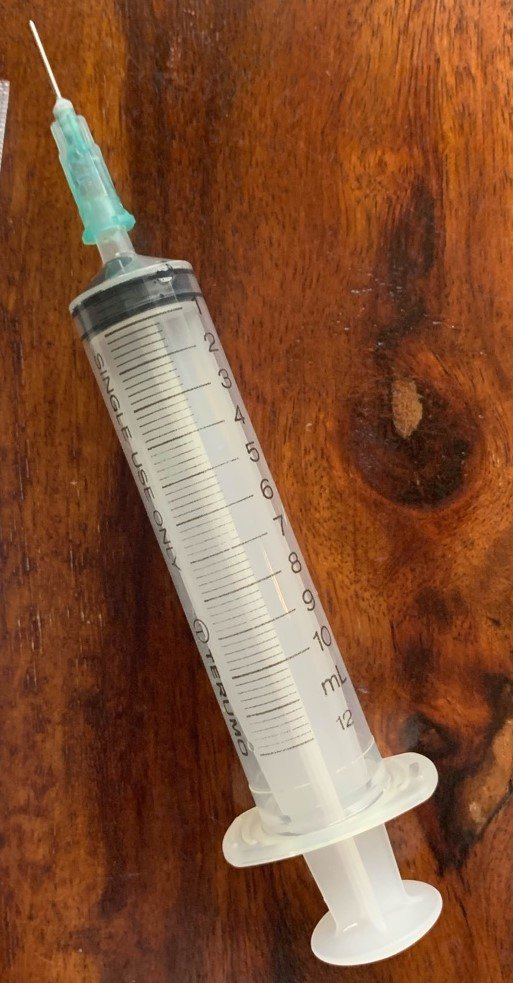
\includegraphics[width = 0.4\columnwidth]{tyusya.jpg}
    \caption{香りを注入する注射器}
    \label{tyusya}
  \end{figure}


\subsection{嗅覚提示実験方法}
 予備実験では香りを閉じこめたゼリーを食べることで,風味を想起させることが出来るかを
検証する.香りを想起させるために香りの感じ方が強い二つの香りを用意した.甘味の強い香り
と塩味が強い香りの香料を使用する.今回の実験では,作成した嗅覚提示ゼリーの有用性を調査
するとともに,中に入れる香りがどの程度の認知を得るか調査した.

\subsection{香料}
香料は甘味の強い香りのバニラと塩味が強い香りの醤油の香料を用意する.香料はコットンに
染み込ませ注射器の中に入れることで気化し香りが充満し,濃度が高い香りを注入することがで
きると考えた.また,今回はゼリーを口の中に入れた際に香りを感じることが出来るかを調査す
るためゼリー自体の味を無味とする.2 名の風邪などひいておらず,鼻詰まりなど匂いを嗅ぐのに
支障がない被験者に実際に香りを注入したゼリーを食べてもらい,風味を感じるか実験を行った.

\subsection{予備実験結果}
被験者 2 名に行った実験の結果,香りを閉じこめたゼリーを食して,バニラの香り,醤油の香
り 2 種類とも風味を僅かに感じたという結果になった.香料の違いでの感覚の差ではなく,香料
の量と濃度がある程度必要なことを示した.また,意見として「無味のゼリーの味が邪魔してい
た」ということから,ゼリーの味付けが無味だと不快感が出てしまうことが明らかになった.
上記の結果から,今回作成したゼリーを用いた嗅覚提示は僅かながら,風味を与える可能性を
感じさせるものである.だが,香りの量,濃度が不十分なため風味が僅かになってしまったため,
香料での香りの出し方と量を増強させる必要があると考える.そのため,コットンに香りをつけ
る量やゼリーの大きさを調整しながら,香りの質を高めることにより感じ方が強化できるのでは
ないかと考えた.また,ゼリー自体の味付けに関して無味だと不快感を感じることから,中に閉
じこめた香りの嗅覚刺激だけでなく,ゼリー自体に甘味や塩味をつけ味覚刺激を与え調査する必
要があると考える.
